\chapter{Introduction}\label{sec:part2}\footnote{This work was published at the 31st ACM SIGKDD conference in 2025:\url{https://dl.acm.org/doi/10.1145/3711896.3736868}}
In this part of the manuscript we design a novel decision tree induction algorithm for supervised learning (\ref{def:sl}) using the MDP formalism.
There already exist works formulating the decision tree induction problem as solving a Markov decision process~\cite{Dulac_Arnold_2011,garlapati2015reinforcementlearningapproachonline,topin2021iterative,chaouki2024branchesfastdynamicprogramming}.
In particular, we showed in the previous part how Topin et al.~\cite{topin2021iterative} could be used to do that using classification POIBMDPs (cf. section~\ref{sec:pomdp-classif}).
We move away from classification POIBMDPs and use a novel MDP formulation that we detail later.
The key differences compared to, e.g.~\cite{topin2021iterative} is that our MDP states are sets of training data rather than feature bounds (cf. definition~\ref{def:cpoibmdp}) and that we dynamically define the set of information gathering actions (cf. definition~\ref{def:ibmdp}).
One other novelty, is that unlike existing works that use reinforcement learning (section~\ref{sec:rl}), we use dynamic programming (\ref{sec:mdp}) to solve exactly decision tree induction formulated as an MDP.

This part of the manuscript is organized as follows.
In this chapter, we motivate the need for new decision tree induction algorithms and present the related works.
In chapter~\ref{sec:dt-mdp}, we introduce a novel MDP formulation of decision tree induction.
Finally, in chapter~\ref{sec:exps-dt}, we show that our new decision tree induction framework performs very well both in terms of training loss and generalization capabilites.

\subsection{Why do we want new decision tree induction algorithms?}
In supervised learning (~\ref{def:sl}), decision trees (\ref{fig:dt}) are valued for their interpretability and performance. 
While greedy decision tree algorithms like CART (algorithm~\ref{alg:cart} \cite{breiman1984classification}remain widely used due to their computational efficiency, they often produce sub-optimal solutions with respect to a regularized training loss (\ref{def:sl}). 
Conversely, optimal decision tree methods can find better solutions but are computationally intensive and typically limited to shallow trees or binary features. We present Dynamic Programming Decision Trees (DPDT), a framework that bridges the gap between greedy and optimal approaches. 
DPDT relies on a Markov decision process (\ref{def:mdp}) formulation combined with heuristic split generation to construct near-optimal decision trees with significantly reduced computational complexity. 
Our approach dynamically limits the set of admissible splits at each node while directly optimizing the tree regularized training loss. Theoretical analysis demonstrates that DPDT can minimize regularized training losses at least as well as CART\@. 
Our empirical study shows on multiple datasets that DPDT achieves near-optimal loss with orders of magnitude fewer operations than existing optimal solvers. 
More importantly, extensive benchmarking suggests statistically significant improvements of DPDT over both CART and optimal decision trees in terms of generalization to unseen data. We demonstrate DPDT practicality through applications to boosting, where it consistently outperforms baselines. 
Our framework provides a promising direction for developing efficient, near-optimal decision tree algorithms that scale to practical applications.

\begin{figure}
    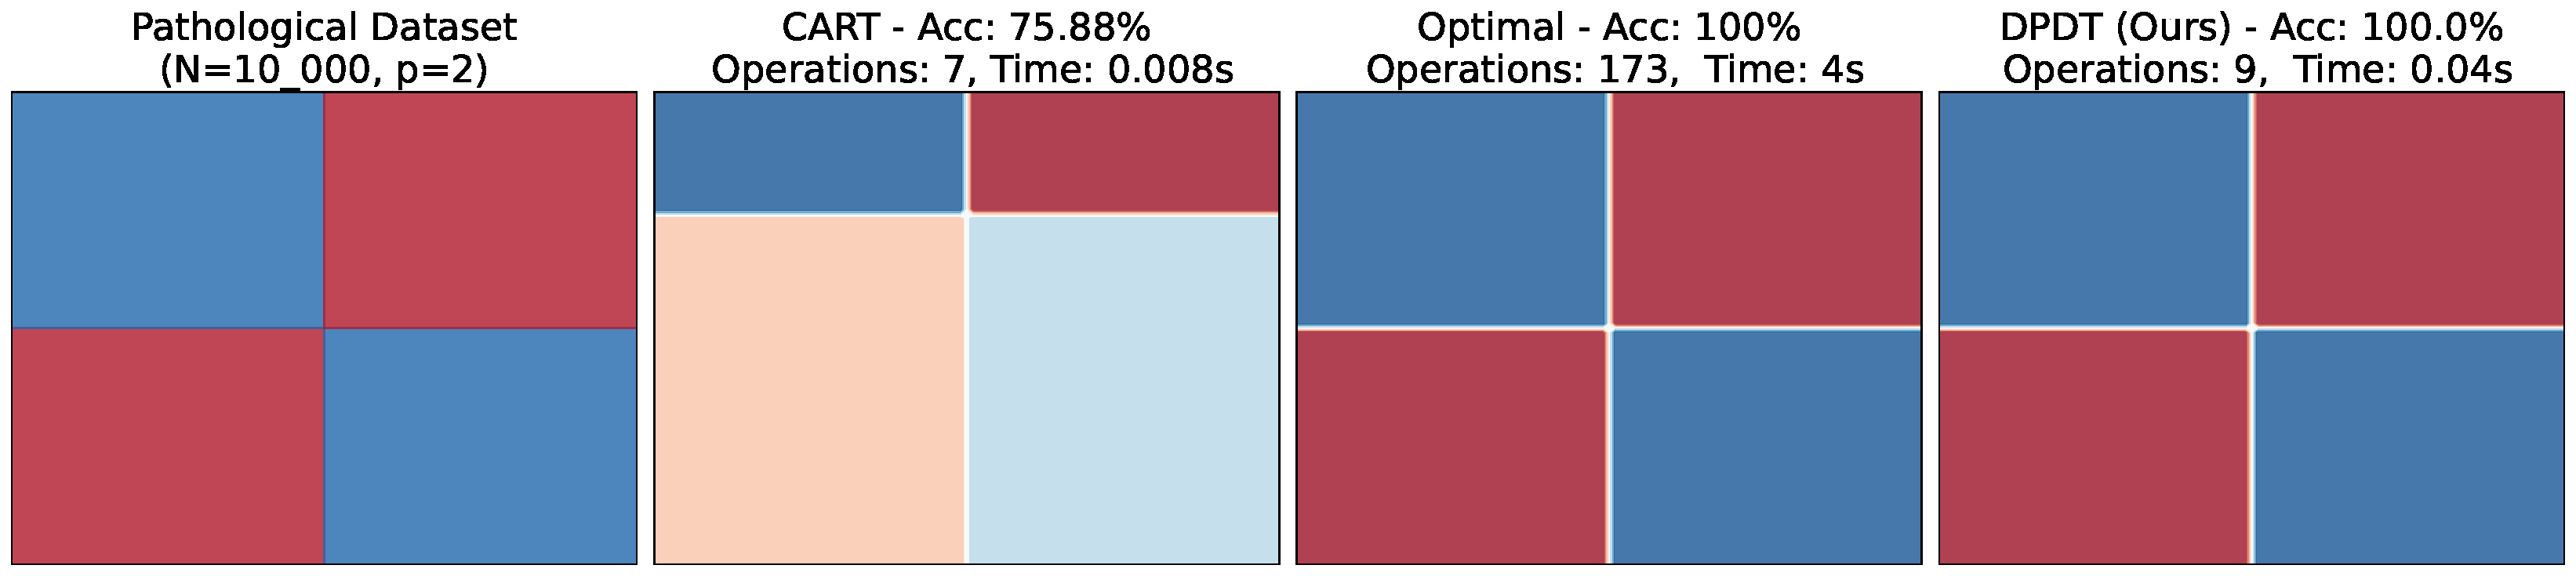
\includegraphics[width=\textwidth]{images/figures/patho_bounds_comparison_checkers.pdf}
    \caption{Pathological dataset and learned depth-2 trees with their scores, complexities, runtimes, and decision boundaries.}
    \label{fig:patho}
\end{figure}

We already saw in the Introduction (\ref{sec:dt}) that decision trees are well studied in supervised learning.
Decision tree inductions algorithms~\cite{ID3,c45,breiman1984classification} are at the core of various machine learning applications. 
Ensembles of decision trees such as tree boosting~\cite{stcohFriedman,FriedmanBoosting,xgb,10.5555/3327757.3327770} are the state-of-the-art for supervised learning on tabular data \cite{grinsztajn2022tree}.

To motivate the design of new decision tree induction algorithms, figure~\ref{fig:patho} exhibits a dataset for which existing greedy algorithms are suboptimal, and optimal algorithms are computationally expensive. 
The dataset is made up of $N=10^4$ samples in $p=2$ dimensions that can be perfectly labeled with a decision tree of depth 2. When running CART, greedily choosing the root node yields a suboptimal tree.
This is because greedy algorithms compute locally optimal splits in terms of information gain. In our example, the greedy splits always give two children datasets which themselves need depth-2 trees to be perfectly split.
On the other hand, to find the root node, an optimal algorithm such as \cite{quantbnb} iterates over all possible splits, that is, $N\times p={20,000}$ operations to find one node of the solution tree.

In this work, we present a framework for designing non-greedy decision tree induction algorithms that optimize a regularized training loss nearly as well as optimal methods. This is achieved with orders of magnitude less operations, and hence dramatic computation savings.
We call this framework ``Dynamic Programming Decision Trees'' (DPDT). For every node, DPDT heuristically and dynamically limits the set of admissible splits to a few good candidates. Then, DPDT optimizes the regularized training loss with some depth constraints.
Theoretically, we show that DPDT minimizes the empirical risk at least as well as CART\@.
Empirically, we show that on all tested datasets, DPDT can reach 99\% of the optimal regularized train accuracy while using thousands times less operations than current optimal solvers. 
More importantly, we follow \cite{grinsztajn2022tree} methodology to benchmark DPDT against both CART and optimal trees on hard datasets. Following the same methodology, we compare boosted DPDT \cite{FREUND1997119} to boosted CART and to some deep learning methods and show clear superiority of DPDT.

\section{Related work}

To learn decision trees, greedy approaches like CART (algorithm~\ref{alg:cart} \cite{breiman1984classification}) iteratively partition the training dataset by taking splits optimizing a local objective such as the Gini impurity or the entropy. 
This makes CART suboptimal with respect to training losses (\ref{def:sl}) \cite{Murthy}. 
But CART remains the default decision tree algorithm in many machine learning libraries such as \cite{scikit-learn,xgb,ke2017lightgbm,9533597} because it can scale to very deep trees and is very fast.
To avoid overfitting, greedy trees are learned with a maximal depth or pruned a posteriori \cite[chapter 3]{breiman1984classification}. 
In recent years, more complex optimal decision tree induction algorithms have shown consistent gains over CART in terms of generalization capabilities \cite{oct,verwer2017learning,murtree}.

Optimal decision tree approaches optimize a regularized training loss while using a minimal number of splits~\cite{oct,mfoct,binoct,quantbnb,murtree,blossom,pystreed,chaouki2024branchesfastdynamicprogramming}.
However, direct optimization is not a convenient approach, as finding the optimal tree is known to be NP-Hard \cite{npcomplete}. Despite the large number of algorithmic tricks to make optimal decision tree solvers efficient~\cite{murtree,quantbnb}, their complexity scales with the number of samples and the maximum depth constraint.
Furthermore, optimal decision tree induction algorithms are usually constrained to binary-features dataset while CART can deal with any type of feature. When optimal decision tree algorithms deal with continuous features, they can usually learn only shallow trees, e.g. Quant-BnB \cite{quantbnb} can only compute optimal trees up to depth 3.
\texttt{PySTreeD}, the latest optimal decision tree library~\cite{pystreed}, can compute decision trees with depths larger than three but uses heuristics to binarize a dataset with continuous features during a pre-processing step. % following for example the Minimum Description Length Principle \cite{MDL}. 
Despite their limitations to binary features and their huge computational complexities, encouraging practical results for optimal trees have been obtained \cite{how-eff,lin2020generalized,costa2023recent,vanderlinden2024optimalgreedydecisiontrees}.
Among others, they show that optimal methods under the same depth constraint (up to depth four) find
trees with 1--2\% greater test accuracy than greedy methods.

In this part, we only consider the induction of non-parametric (cf. section~\ref{related-work-pomdp}) binary depth-constrained axis-aligned trees. 
We write this model class $\mathcal{T}_D$ where $D$ is the maximum tree depth.
Axis-aligned tree nodes only test one data feature only against one thresholds only as opposed to e.g. oblique trees~\cite{murthy1994system}.
In our definition (\ref{sec:dt}), this means that we only consider Boolean functions $(j, \mathbb{R}):\rightarrow \{0, 1\}$ (the careful reader might notice the clear similarity with information gathering actions in IBMDPs (definition~\ref{def:ibmdp},~\cite{topin2021iterative})).
Like for the reinforcement learning setting, there exists a line of work on parametric trees: Tree Alternating Optimization (TAO) algorithm~\cite{NEURIPS2018_185c29dc,9534446,10.1145/3412815.3416882} that only optimizes tree nodes threshold values for fixed nodes features similarly to optimizing neural network weights with gradient-based methods. 

Now we write explicitely the supervised learning objective (\ref{def:sl}) for decision trees:

\begin{definition}[Supervised learning of decision trees (decision tree induction)]\label{eq:suplearning}
    Assume that we have access to a set of $N$ examples denoted $\mathcal{E} = {\{(x_i, y_i)\}}_{i=1}^N$. Each datum $x_i$ is described by a set of $p$ features. $y_i \in {\mathcal Y}$ is the label associated with $x_i$.
    \begin{align*}
    T^* &= \underset{T \in \mathcal{T}_D}{\operatorname{argmin}}\ \frac{1}{N}\overset{N}{\underset{i=1}{\sum}}{l}(y_i, T(x_i)) + \alpha C(T) \\
    T^* &= \underset{T \in \mathcal{T}_D}{\operatorname{argmin}}\ {\mathcal L}_\alpha(T)
\end{align*}
where $C: \mathcal{T}_D \rightarrow \mathbb{R}$ is a complexity penalty that helps prevent or reduce overfitting such as the number of nodes~\cite{breiman1984classification,quantbnb}, or the expected number of splits to label a data\cite{how-eff}. The complexity penalty is weighted by $\alpha \in [0, 1]$. %For regression problems where $\mathcal{Y} \subset \mathbb R$, we use the squared error $l(y_i, T(x_i)) = {(y_i - T(x_i))}^2$. 
\end{definition}

In the rest of this part we focus on classification tasks: we use the 0--1 loss $l(y_i, T(x_i)) = 1_{\{y_i\neq T(x_i)\}}$.
Please note while we focus on classification tasks, our framework extends naturally to regression tasks.

In the supervised learning setting, there exist many other areas of decision tree research \cite{loh2014fifty} such as inducing non-axis parallel decision trees \cite{murthy1994system,10.1145/3637528.3671903}, splitting criteria of greedy trees \cite{vanderlinden2024optimalgreedydecisiontrees}, different optimization of parametric trees \cite{NIPS2015_1579779b,10.5555/3327757.3327770}, or pruning methods \cite{pruning1,pruning2}. 